\section{Experimental Setting}
\label{subsec:exp_setup}

\textbf{Models and budgets.}
We mainly distill Llama-3.3-70B-Instruct into Llama-3.1-8B-Instruct, and report
Qwen2.5-72B-Instruct to Qwen2.5-14B-Instruct results in
Appendix~\ref{sec:app_experiment}. All methods use the same student checkpoint,
training recipe, and $20$M/$150$M distillation-token budgets.

\textbf{Evaluation protocol.}
We evaluate eight capabilities using Appendix
Table~\ref{tab:capabilities-benchmarks}. For each benchmark, 10\% of non-test
data is used for profiling, requirement inference, and allocation updates; the
held-out split is reserved for final reporting. Generation uses temperature $0$
with the same prompt template across methods. We report mean $\pm$ standard
deviation over three seeds.

\textbf{Baselines.}
For each capability, we build a held-out-filtered distillation pool from its
benchmark prompts. For multi-dataset capabilities, we use balanced dataset-level
sampling. The six main baselines combine three teacher signals---final response
(Resp), chain-of-thought plus response (CoT), and token-level logits (Logit)---
with two objectives, SFT and KD. Each baseline is one-hot at the capability
level, spending the full budget on the target-capability pool.
\rev{We also compare against four allocation baselines that share ReAD's
generator, teacher, and budget and differ only in how $\mathbf{w}_t$ is chosen
(Table~\ref{tab:budget_diagnostics}): \emph{Uniform static}
($\mathbf{w}_t=\mathbf{1}/|\mathcal{C}|$), \emph{Task-static mix}
($\mathbf{w}_t=\mathbf{r}_\tau$), \emph{Greedy one-step} (re-selects
$\mathbf{w}_t$ each step by the ensemble mean alone, $\kappa=0$), and
\emph{Grid-searched} (best fixed allocation in $\mathcal{A}(\tau)$ on the
profiling split). These are the matched reference points for adaptive allocation.}

\textbf{ReAD implementation.}
ReAD runs for $20$ decision steps, with bandit updates, proxy refreshes, and data
resampling every $1.0$M tokens in the $20$M setting and every $7.5$M tokens in
the $150$M setting. Proxy refresh adds 3.12\% wall-clock overhead, the full online loop adds
5.63\%, and the reusable requirement identifier costs 3.79 GPU-hours to train
once.
\rev{\textbf{Cost accounting.} $B$ counts the teacher-generated tokens the
student is trained on and is identical for all methods. Two ReAD-specific costs
fall outside $B$ and are reported separately rather than folded into it: the
identifier is trained once from auxiliary tasks and reused for every task and
budget, so its 3.79 GPU-hours are amortized, and the fixed probe suite is the
3.12\% overhead above.}


\section{Experiments}
\label{sec:exp}

We study four questions: \textbf{RQ1} utility gains under the same budget;
\textbf{RQ2} reduced waste and spillover; \textbf{RQ3} the value of adaptive
bandit scheduling over static or greedy alternatives; and \textbf{RQ4}
transfer beyond capability-aligned benchmarks.

\begin{table*}[t]
\centering
\tiny
\setlength\tabcolsep{1pt}
\caption{Capability profile under a 20M-token budget on Llama. ReAD achieves the strongest average profile while using the same student initialization and token budget as all baselines.}
\begin{tabular}{lcccccccc}
\toprule
\textbf{Method} &
\textbf{General} &
\textbf{Steer.} &
\textbf{Reason.} &
\textbf{Math} &
\textbf{Code} &
\textbf{Tool} &
\textbf{LCU} &
\textbf{Multi.} \\
\midrule
Teacher only &
$48.13\pm0.35$ & $89.98\pm0.40$ & $10.51\pm0.12$ & $48.34\pm0.55$ &
$88.40\pm0.70$ & $31.90\pm0.45$ & $36.20\pm0.40$ & $91.10\pm0.55$ \\
Student only &
$31.09\pm0.40$ & $49.22\pm0.55$ & $8.72\pm0.15$ & $15.56\pm0.60$ &
$72.60\pm0.95$ & $25.83\pm0.60$ & $30.40\pm0.45$ & $68.90\pm0.80$ \\
\midrule
Resp-SFT & $33.28\pm0.47$ & $52.84\pm0.71$ & $9.05\pm0.18$ & $17.12\pm0.83$ & $74.06\pm1.09$ & $26.92\pm0.78$ & $31.28\pm0.51$ & $70.02\pm0.93$ \\
CoT-SFT & $33.02\pm0.52$ & $52.16\pm0.76$ & $9.46\pm0.14$ & $18.58\pm0.77$ & $73.82\pm1.02$ & $26.81\pm0.74$ & $31.19\pm0.57$ & $69.78\pm0.88$ \\
Logit-SFT & $33.61\pm0.44$ & $53.04\pm0.69$ & $9.12\pm0.17$ & $17.63\pm0.79$ & $74.48\pm1.15$ & $27.03\pm0.70$ & $31.42\pm0.53$ & $70.21\pm0.90$ \\
Resp-KD & $33.83\pm0.50$ & $53.62\pm0.73$ & $9.18\pm0.16$ & $17.84\pm0.74$ & $74.23\pm1.07$ & $27.18\pm0.76$ & $31.58\pm0.55$ & $70.48\pm0.95$ \\
CoT-KD & $33.46\pm0.46$ & $52.98\pm0.78$ & $9.62\pm0.13$ & $19.34\pm0.72$ & $74.03\pm1.10$ & $27.06\pm0.72$ & $31.47\pm0.58$ & $70.08\pm0.89$ \\
Logit-KD & $34.02\pm0.43$ & $54.21\pm0.66$ & $9.25\pm0.15$ & $18.20\pm0.76$ & $74.62\pm1.12$ & $27.41\pm0.69$ & $31.72\pm0.50$ & $70.81\pm0.91$ \\
\midrule
\textbf{ReAD} &
$\mathbf{35.02\pm0.41}$ & $\mathbf{58.03\pm0.61}$ & $\mathbf{10.01\pm0.12}$ & $\mathbf{21.06\pm0.68}$ &
$\mathbf{77.06\pm0.97}$ & $\mathbf{29.82\pm0.64}$ & $\mathbf{33.58\pm0.49}$ & $\mathbf{73.04\pm0.84}$ \\
\bottomrule
\end{tabular}
\label{tab:llama_20m}
\end{table*}

\begin{figure}[t]
  \centering
  
\includegraphics[width=\columnwidth]{figure/rq2_legend.pdf}
  \vspace{-1.5em}

  \begin{subfigure}[t]{0.24\columnwidth}
    \centering
    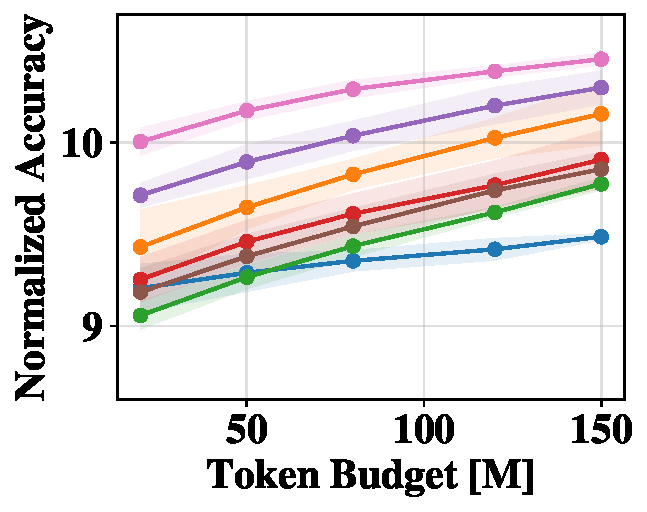
\includegraphics[width=\linewidth]{figure/rq2_lineplot_reasoning.pdf}
    \caption{Reasoning}
    \label{fig:r2_reason}
  \end{subfigure}
  \hfill
  \begin{subfigure}[t]{0.24\columnwidth}
    \centering
    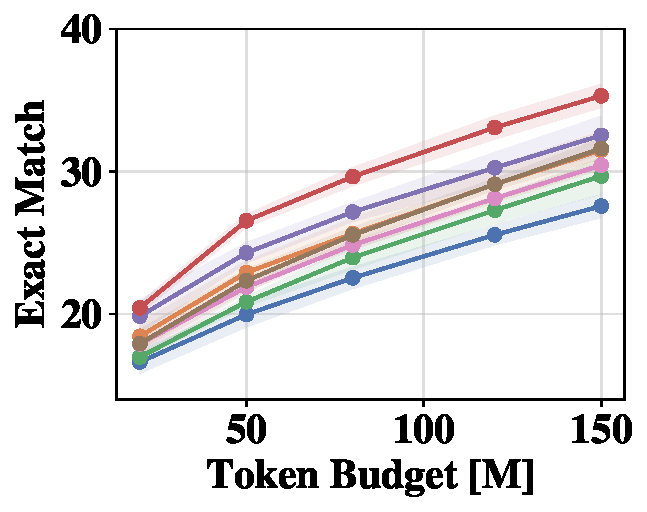
\includegraphics[width=\linewidth]{figure/rq2_lineplot_math.pdf}
    \caption{Math}
    \label{fig:r2_math}
  \end{subfigure}
  \hfill
  \begin{subfigure}[t]{0.24\columnwidth}
    \centering
    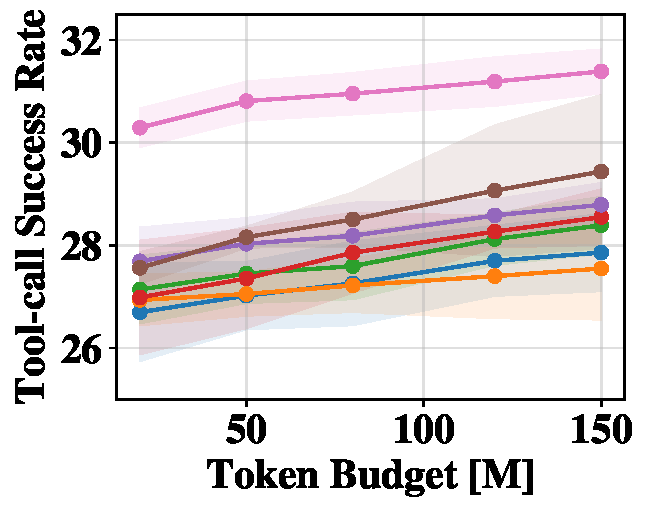
\includegraphics[width=\linewidth]{figure/rq2_lineplot_tool_use.pdf}
    \caption{Tool Use}
    \label{fig:r2_tool}
  \end{subfigure}
  \hfill
  \begin{subfigure}[t]{0.24\columnwidth}
    \centering
    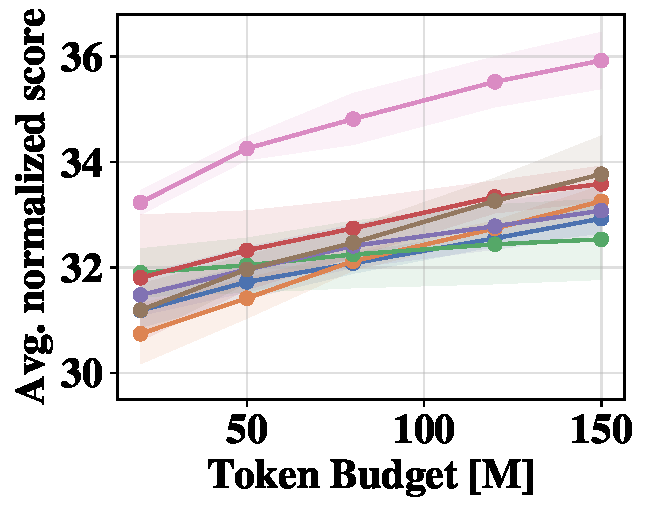
\includegraphics[width=\linewidth]{figure/rq2_lineplot_lcu.pdf}
    \caption{LCU}
    \label{fig:r2_lcu}
  \end{subfigure}

  \caption{Performance versus token budget for four bottleneck capabilities. Curves show mean $\pm$ standard deviation over three seeds.}
  \label{fig:rq2_budget}
  \vspace{-0.8em}
\end{figure}

\subsection{Results and Analysis}
\label{subsec:exp_results}

\paragraph{RQ1: Utility under a fixed budget.}
Table~\ref{tab:llama_20m} shows that ReAD achieves the strongest capability
profile at $20$M tokens\rev{, outperforming the six one-hot baselines on every
capability}. The gains
are especially pronounced on bottleneck capabilities such as Steerability, Math,
Tool Use, and LCU. \rev{Since each one-hot baseline spends the whole budget on one capability,
this isolates the value of distributing the budget at all; the matched
comparison for \emph{how} to distribute it is Table~\ref{tab:budget_diagnostics}(b) (RQ3).} The $150$M Llama results and Qwen results in
Appendix~\ref{sec:app_experiment} show the same ordering, suggesting that the
improvement is not tied to a single teacher--student pair.

\paragraph{RQ2: Budget efficiency.}
Figure~\ref{fig:rq2_budget} reports budget-scaling curves for Reasoning, Math,
Tool Use, and LCU. ReAD achieves higher performance at the same budget and
maintains the strongest scaling trend, indicating that adaptive allocation
reduces wasted tokens on low-marginal-return updates.

\begin{table}[t]
  \centering
  \captionsetup{font=small, width=0.96\linewidth, skip=3pt}
  \caption{\rev{\textbf{Budget-allocation diagnostics.} (a) 150M-token
gain--spillover trade-off from the capability transfer matrix: ReAD keeps
near-best on-target gain with much less off-target degradation. (b)
Matched-budget allocation schedules under the same generator.}}
  \label{tab:budget_diagnostics}
  \vspace{-0.4em}

  \footnotesize
  \setlength{\tabcolsep}{2.2pt}
  \renewcommand{\arraystretch}{0.94}

  \begin{subtable}[t]{0.55\linewidth}
    \centering
    \caption*{\textbf{(a) Harmful transfer at 150M}}
    \begin{tabular}{@{}lccc@{}}
      \toprule
      \textbf{Method} & \textbf{On-tgt $\uparrow$} & \textbf{Off-tgt $\Delta\uparrow$} & \textbf{Neg. $\downarrow$} \\
      \midrule
      Single-cap. KD
        & $\mathbf{4.79{\pm}0.29}$
        & $-1.57{\pm}0.21$
        & $0.43{\pm}0.03$ \\
      Task-static mix
        & $4.61{\pm}0.25$
        & $-0.87{\pm}0.17$
        & $0.29{\pm}0.03$ \\
      Greedy one-step
        & $4.72{\pm}0.23$ % placeholder: replace with measured value
        & $-0.94{\pm}0.19$ % placeholder: replace with measured value
        & $0.31{\pm}0.03$ % placeholder: replace with measured value
        \\
      Grid-searched
        & $4.66{\pm}0.24$ % placeholder: replace with measured value
        & $-0.71{\pm}0.16$ % placeholder: replace with measured value
        & $0.25{\pm}0.03$ % placeholder: replace with measured value
        \\
      \textbf{ReAD}
        & $4.79{\pm}0.24$
        & $\mathbf{-0.38{\pm}0.12}$
        & $\mathbf{0.17{\pm}0.02}$ \\
      \bottomrule
    \end{tabular}
  \end{subtable}
  \hfill
  \begin{subtable}[t]{0.42\linewidth}
    \centering
    \caption*{\textbf{(b) Allocation schedules}}
    \begin{tabular}{@{}lcc@{}}
      \toprule
      \textbf{Method} & \textbf{20M $\uparrow$} & \textbf{150M $\uparrow$} \\
      \midrule
      Uniform static
        & $60.94{\pm}0.48$
        & $64.73{\pm}0.36$ \\
      Task-static mix
        & $61.71{\pm}0.43$
        & $65.52{\pm}0.33$ \\
      Greedy one-step
        & $62.03{\pm}0.41$
        & $66.01{\pm}0.30$ \\
      Grid-searched
        & $61.88{\pm}0.42$
        & $65.81{\pm}0.31$ \\
      \textbf{ReAD}
        & $\mathbf{63.04{\pm}0.39}$
        & $\mathbf{67.21{\pm}0.28}$ \\
      \bottomrule
    \end{tabular}
  \end{subtable}

  \vspace{-1.6em}
\end{table}

\paragraph{RQ2: Gain--spillover trade-off.}
Table~\ref{tab:budget_diagnostics}(a) shows that ReAD improves the
gain--spillover trade-off. Single-capability KD achieves strong target gains but
causes larger off-target degradation, while static mixing reduces spillover at
the cost of weaker target improvement. ReAD better balances the two: it keeps
strong on-target gains while suppressing negative transfer across
non-target capabilities.

\paragraph{RQ3: Adaptive scheduling.}
Table~\ref{tab:budget_diagnostics}(b) compares ReAD with stronger allocation
baselines under the same generator and token budgets. Static schedules cannot
adapt once marginal returns and spillover change during training, while the
greedy heuristic ignores uncertainty and remaining budget. ReAD outperforms
both, with a larger margin at $150$M where saturation and spillover are stronger.
\rev{These margins are smaller than those over one-hot baselines ($+1.0$/$+1.2$
over Greedy one-step and $+1.2$/$+1.4$ over Grid-searched at $20$M/$150$M, with
seed standard deviations of $0.3$--$0.4$), as every allocation baseline already
mixes capabilities; the remaining gain is the value of re-estimating the mix as
the student and the remaining budget change.}

\begin{wrapfigure}[8]{r}{0.42\textwidth}
  \vspace{-1.6em}
  \centering
  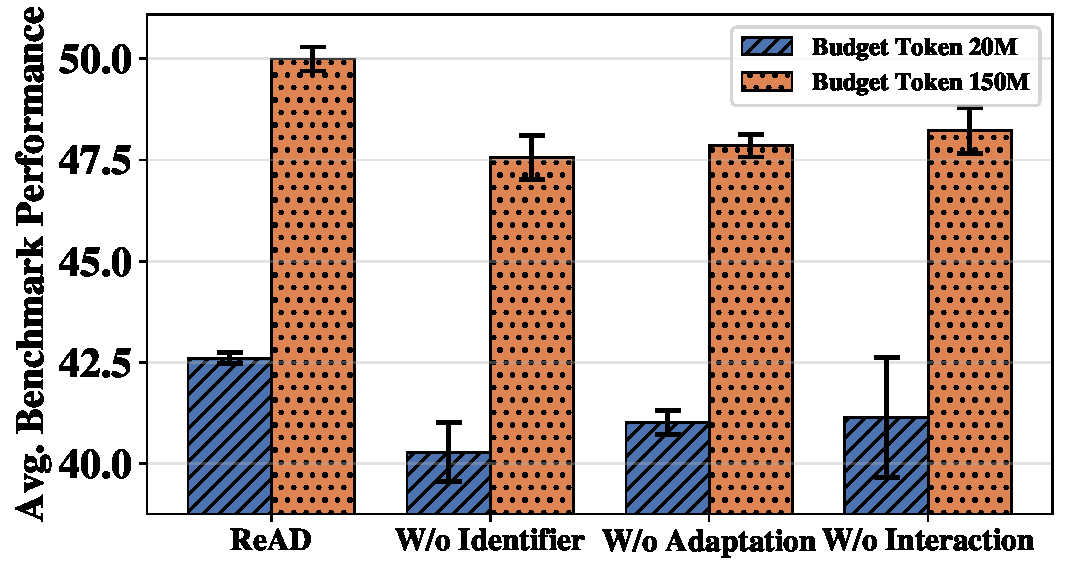
\includegraphics[width=0.40\textwidth]{figure/rq3_ablation_avgmetric_20m_150m.pdf}
  \caption{Ablation of ReAD components.}
  \label{fig:rq3_ablation}
  \vspace{-1.4em}
\end{wrapfigure}

\paragraph{Component ablation.}
We ablate ReAD by removing one component while fixing the teacher, student,
prompt pools, training recipe, and budget. Removing requirement identification
makes the allocation uniform; removing adaptation uses a fixed allocation; and
removing interaction awareness drops the spillover penalty.
Figure~\ref{fig:rq3_ablation} shows that identification and adaptation drive the
largest gains, while interaction modeling provides additional improvement by
reducing harmful transfer.

\paragraph{RQ4: Transfer beyond aligned benchmarks.}
Finally, we evaluate ReAD on held-out XSTest~\citep{rottger2024xstest} using the same requirement
identifier and allocation pipeline without adding a new capability head. ReAD
improves both safe-refusal and unsafe-refusal metrics over the best SFT/KD
baseline; full results are reported in Appendix Table~\ref{tab:xstest}.